AD\documentclass[a4paper,10pt]{article}

% Import packages here
\usepackage[utf8]{inputenc}
\usepackage{graphicx}

% Title
\title{Muonium - Encrypted cloud storage}
\author{Paul Feuvraux}


\begin{document}
\maketitle

DRAFT


\section{Introduction}
This paper aims to explain the technical side of \emph{Muonium}, a fully open source encrypted cloud storage.


Muonium aims to protect users' online privacy through \emph{End-to-End Encryption} against malicious parties. Muonium automatically encrypts user's data, uploads and stores them on the cloud. Users can have access to their encrypted files anytime, anywhere.

\section{Terms}
In this section, we define all technical terms used throughout the paper.

\begin{itemize}
    \item \textbf{Content Encryption Key ($CEK$)}:
        Alphanumeric UTF-8 randomly generated string. It is used in the Key derivation function.
    \item \textbf{Passphrase ($P$)}:
        User's defined alphanumeric UTF-8 passphrase during registration on the client side.
    \item \textbf{File Encryption Key (FEK)}:
        256-bit symmetric key derived from $CEK$. We use $FEK$ to encrypt/decrypt files. Each file has its own FEK.
    \item \textbf{Login Password $LP$}: Used for authentication procedures
    \item \textbf{Hash function}: We use SHA-384 at the client-side and Blowfish with 192-bit of Salt at the server-side.
    \item \textbf{Key derivation function:} Every key derivation is performed with PBKDF2. We denote this process as $KDF(P)$ where $P$ is the user's passphrase.
    \item \textbf{Symmetric encryption}: We use AES-256 over GCM.
        We denote this process as $Enc(k,x)$ where $k$ is a symmetric key and $x$ is the plain-text to be encrypted.
    \item \textbf{Symmetric decryption}: We use AES-256 over GCM;
        We denote this process as $Dec(k, x)$ where $k$ is a symmetric key and $x$ is the encrypted text to be decrypted.
		\item \textbf{Asymmetric encryption}: We use a 4096-bit public key, and is denoted as $AsymEnc(pubkey, content)$.
		\item \textbf{Asymmetric decryption}: We use a 4096-bit private key, and is denoted as $AsymDec(privkey, content)$.
\end{itemize}

\section{Protocol}
\subsection{Registration}
Users must register with a Muonium server in order to use its service. During this process, the user has to provide:

\begin{itemize}
    \item \textbf{Email address}: Used for authentication procedures.
    \item \textbf{User name}: Used as an email address alternative for authentication procedures.
    \item \textbf{Login Password $LP$}:
    \item \textbf{Passphrase $P$}: Used in the cryptographic system.
\end{itemize}

The \emph{user name} and the user's \emph{email address} are stored in plain text in the database while the Login Password $LP$ is double-hashed a first time at the client-side under SHA-384 and a second time at the server-side under Blowfish (described in figure \ref{Fig:fig1}).

\begin{figure}[!h]
\centering
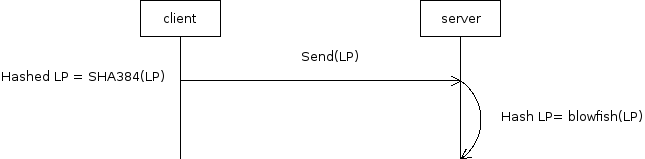
\includegraphics[width=0.8\textwidth]{diagram/figure1}
\caption{$LP$ is hashed and stored on the server}
\label{Fig:fig1}
\end{figure}

While the user submits his credentials, Muonium client generates a $CEK$, encrypts it with $P$ and sends along with the user's credentials to the server as follow.

Explain Figure \ref{Fig:fig2}

\subsection{Connection}
To use the service, an user must establish a connection with a Muonium server. There are two steps involved: \emph{Authentication} and \emph{$CEK$ decryption}.

\subsubsection{Authentication}
The user types in his credentials (user name/email address and $LP$) plus his passphrase $P$. Muonium server then verify these information.

\subsubsection{$CEK$ decryption}
Once the user is authenticated, Muonium server return $Enc(P, CEK)$. It is then decrypted as $Dec(P, CEK)$. Client stores $CEK$ locally on ...

Diagram for both subsubsection

\subsection{Upload}
\subsubsection{Key derivation}
To proceed to a key derivation, a Salt is generated on 128 bits. We use a strengthening by a factor of 7000. The output will be a 256-bit symmetric key. Such as $FEK = KDF(CEK, Salt, 7000, 256)$ where 7000 (strengthening by factor) and 256 (symmetric key output size) are constants.

\subsubsection{Splitting}
A file is split in 1Mo chunks. For each chunk are generated an initialization vector ($IV$) and authentication data  ($AD$), both are generated on 128 bits.

\subsubsection{Encryption}
For every chunk an encryption is performed with the $IV$ and $AD$ of the chunk itself and the $FEK$ of the file such as $Enc(FEK, Chunk, IV, AD, 128)$ where 128 is a constant which represent the tag length.

\subsubsection{Encapsulation}
Every chunk is encapsulated with the AD and IV such as $chunk_packet=(AD||IV||encrypted_chunk)$.

\subsubsection{Uploading process}
Once encapsulated, the chunk is sent to the server. All chunks are sent one by one.



\subsection{Decryption}
\subsubsection{Extraction}
The first chunk of the remote file is downloaded. We extract the $IV$, $AD$, and Salt from it.

\subsubsection{Key derivation}
The Salt is used to proceed to a key derivation, such as $KDF(CEK, Salt, 7000, 256)$, the output will be the $FEK$ of the file.

\subsubsection{Decryption}
The content of the first chunk ($DATA$) is decrypted with the extracted cryptographic parameters such as $Dec(FEK,DATA,IV,AD,128)$. The other chunks are decrypted with their own extracted cryptographic parameters and the same $FEK$ as the first chunk.

\subsubsection{Reassembling}
For each chunk belonging to the same file, it is written in a remote file.
\medskip

\subsection{File sharing}
Users can share files, internally (between Muonium users) and externally (via an external link).

\subsubsection{External file sharing}

\textbf{Encryption.}

The user choose to share his/her file with another Muonium user.

When the file is shared, the first chunk of the file is downloaded in order to extract the salt, which will
be used to rebuild the $FEK$ of the file such as $KDF(CEK, salt, 7000, 256)$. Once the $FEK$ rebuilt,
a new $salt_d_k$ is randomly generated in order to derive the $FEK$ into a derivation key $DK$. Then,
we proceed to a key derivation such as $DK=KDF(p, salt_d_k, 7000, 256)$, where $p$ is the passphrase
that the user had to type to share it with external users (people who don't use Muonium).

In order to encrypt $FEK$, an $IV$ and $AT$ are randomly generated on 128 bits.

Then, the encryption is processed such as $FEK_c=Enc(DK, FEK, IV, AD, 128)$, where $FEK_c$ is the
encrypted $FEK$. Once the $FEK$ got encrypted, the cryptographic parameters are encapsulated with
$FEK_c$ such as $packet=(FEK_c||salt||IV||AD)$.

\textbf{Decryption.}

An external user goes to the public link, type the passphrase, and download the file.

$packet$ is obtained from the database and sent to the external user. The user types the passphrase
$p$. We extract $salt_d_k$ from $packet$ and proceed to a key derivation such as $DK=(p, salt, 7000, 256)$.

Once $DK$ obtained from the key derivation process, we extract $IV$ and $AD$ from $packet$ and proceed to
the decryption of $FEK_c$ to get $FEK$ such as $FEK=Dec(DK, FEK_c, IV, AD)$.

Once $FEK$ obtained, every chunk of the file is downloaded, decrypted, and reassembled to recreate the
decrypted file.

\subsubsection{Internal file sharing}

Internal file sharing uses asymmetric encryption, thus, the user needs to generate their pair of
keys if it has not been done before. Asymmetric keys aren't generated at the registration. Asymmetric
keys are generated on 4096 bits.

\textbf{Encryption.}

The user types the username of the user they want to share the file with. If a match is found, then the
shared-with user's public key $pubkey_u$ is downloaded to the client.

First of all, the first chunk of the file is downloaded, and we extract its $salt$ in order to proceed
to a key derivation for rebuilding $FEK$ such as $FEK=KDF(CEK, salt, 7000, 256)$.

Once the $FEK$ obtained, we proceed to the encryption of it such as $FEK_c=AsymEnc(pubkey_u, FEK)$, then
$FEK_c$ is sent to the server and is stored in the database.

\textbf{Decryption.}

The user click on "shared with me", downloads the file, and gets their private key $priv_u$.

The client gets $FEK_c$ from the database, and decrypts it such as $FEK=AsymDec(priv_u, FEK_c)$.

Once $FEK$ obtained, every chunk of the file is downloaded, decrypted, and reassembled to recreate the
decrypted file.

\section{Conclusion}
Muonium is based on the end-to-end encryption model, consequently nobody can access a user's data except the user himself.

\section{Notes}

\begin{itemize}
	\item \textbf{Key derivation algorithm}: it exists several improved key derivation
	algorithms, but we've chosen to use PBKDF2 for its performances and safety.
	\item \textbf{FEK leaks}: when an external or internal user gets to be shared a file with,
	they get to know $FEK$, which means that they would be able to leak it publicly. Hence,
	it is recommended to re-upload the file once the user gets done to share it.
\end{itemize}


\section{Thanks to}

\textbf{Hoang Long Nguyen}, for your help at writing this whitepaper.

\bibliographystyle{unsrt}%Used BibTeX style is unsrt
\bibliography{sample}

\end{document}
